\section{Introduction}


\begin{figure*}[t]
  \centering

  \subfloat[Church (left) and obelisks (center and right).]
    {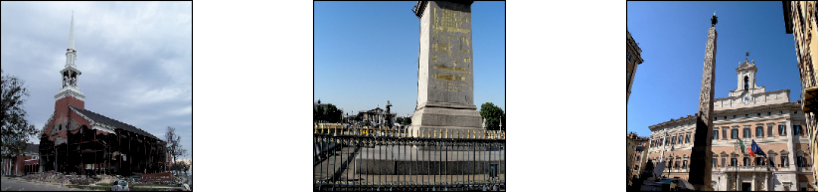
\includegraphics[width=.95\textwidth]{figs/qualitative_images.png}}

  \subfloat[The CNN probability distributions of the images above.]
    {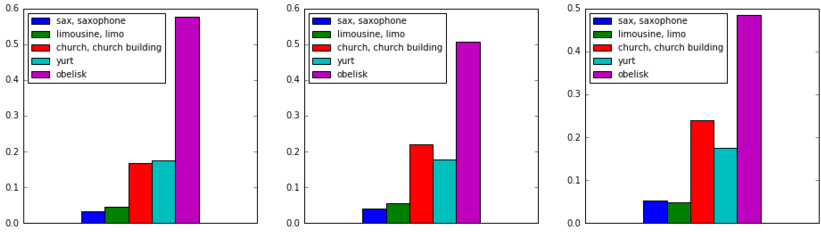
\includegraphics[width=.95\textwidth]{figs/qualitative_probs.png}}

  \caption{
    The CNN gives higher probability values to objects which visually similar to
    the ground truth. Here, the classifier predicted that the images were
    \emph{obelisk}. These examples show visual similarities between
    \emph{church} and \emph{obelisk}. These categories are also similar
    semantically.
  }
  \label{fig:qualitative_results}
\end{figure*}


Deep neural networks have been very popular in recent years due to their high
capacity and strong generalization abilities.  Convolutional neural networks
(CNNs) have been especially popular in computer vision for image classification.
However, despite their empirical success, training a deep learning model
generally requires a massive amount of data, often in the order of millions of
images. Such large amounts of labeled data are expensive to obtain. Hence 
improvements which result in decreasing the number of labeled examples to train
a high performing CNN would dramatically reduce the human component of the
training process.

Because of the high computational cost of training and even evaluating new data
on deep neural networks, \cite{hinton2015distilling} explored a new method
for transfering the learned weights of a large, expert deep neural network model
(i.e. a model with a large number of parameters) to a simpler one (with
significantly fewer parameters) by training the simpler model with \emph{soft
labels} produced by the expert model. They showed that this can reduce the
amount of training data needed by the simpler model while still producing
comparable results, and because it has fewer parameters, it is able to evaluate
data faster.

We attempt to approximate the soft labels produced by the expert network in
\cite{hinton2015distilling} \emph{cheaply} by leveraging existing sources of
data which can be used to compute \emph{similarities} between labels, and allows
for a soft labeling scheme to be used.  We show that this augmented learning
signal results in improved classification results over a model trained with a
one-hot learning signal. By consequence, such models can be trained with a
smaller amount of data to achieve comparable performance, thus the time to train
such a model can be significantly reduced.
Figure \ref{fig:qualitative_results} shows an example of how visual and semantic
similarity are related.

%Finally, by reducing the amount of required training data, we hope to show that
%our technique can be applied to domains where labeled training examples are
%limited, which may have previously prevented deep learning techniques from being
%used in those settings.

%% This is more related works:
%There has been a lot of work done in studying the relationship between vision
%and language, showing that it is possible to integrate linguistic information
%to improve visual classification tasks \cite{izadinia2015segment,
%frome2013devise, marszalek2007semantic, grauman2011learning}.
%Studies have shown that there are correlations between visual and semantic
%similarities among visual object categories \cite{deselaers2011visual}.
%Thus, we believe that we can achieve a performance gain and/or reduce the
%amount of required training images, as was done in \cite{hinton2015distilling},
%but using linguistic information instead of relying on the learned weights of a
%stronger deep model.
